\section{Evoluzione di YOLO}
YOLO ha subito un'evoluzione significativa nel corso degli anni, con ogni nuova versione che ha introdotto importanti miglioramenti in termini di precisione, velocità e capacità di generalizzazione.

\subsection{YOLOv1}
La prima versione di YOLO, proposta nel 2016\cite{14}, è composta da una singola rete neurale convoluzionale che processa l'intera immagine di input in un singolo passaggio. Nella rete troviamo le seguenti tipologie di layers:
\begin{itemize}
  \item \textbf{Convolutional Layers}: Applicano convoluzioni con filtri di diverse dimensioni per estrarre feature di alto livello dall'immagine di input. Questi strati sono responsabili della rilevazione dei pattern, come bordi, texture e forme complesse.
  \item \textbf{Max-Pooling Layers}: Ridimensionano le feature map riducendo la risoluzione spaziale, mantenendo le feature più importanti e riducendo la quantità di parametri e il costo computazionale. Max-pooling seleziona il valore massimo in ogni finestra del filtro, riducendo così l'informazione spaziale ma conservando le feature dominanti.
  \item \textbf{Fully Connected (FC) Layers}:  Connettono ogni unità di un layer a tutte le unità del layer successivo, combinando le feature estratte per produrre le predizioni finali. Questi strati sono utilizzati per la classificazione finale e la regressione delle bounding box.
\end{itemize}

L'architettura di YOLOv1 si ispira a GoogLeNet (rete nota per i suoi moduli inception che permettono di utilizzare filtri di diverse dimensioni in parallelo) e utilizza 24 convolutional layers per estrarre feature rilevanti a vari livelli di astrazione, alternati a max-pooling layers per ridurre la dimensione spaziale delle feature maps, mantenendo al contempo le informazioni più important. Successivamente, 2 FC layers combinano queste feature estratte per predire le bounding box e le probabilità di classe.


\begin{figure}[ht]
    \centering
    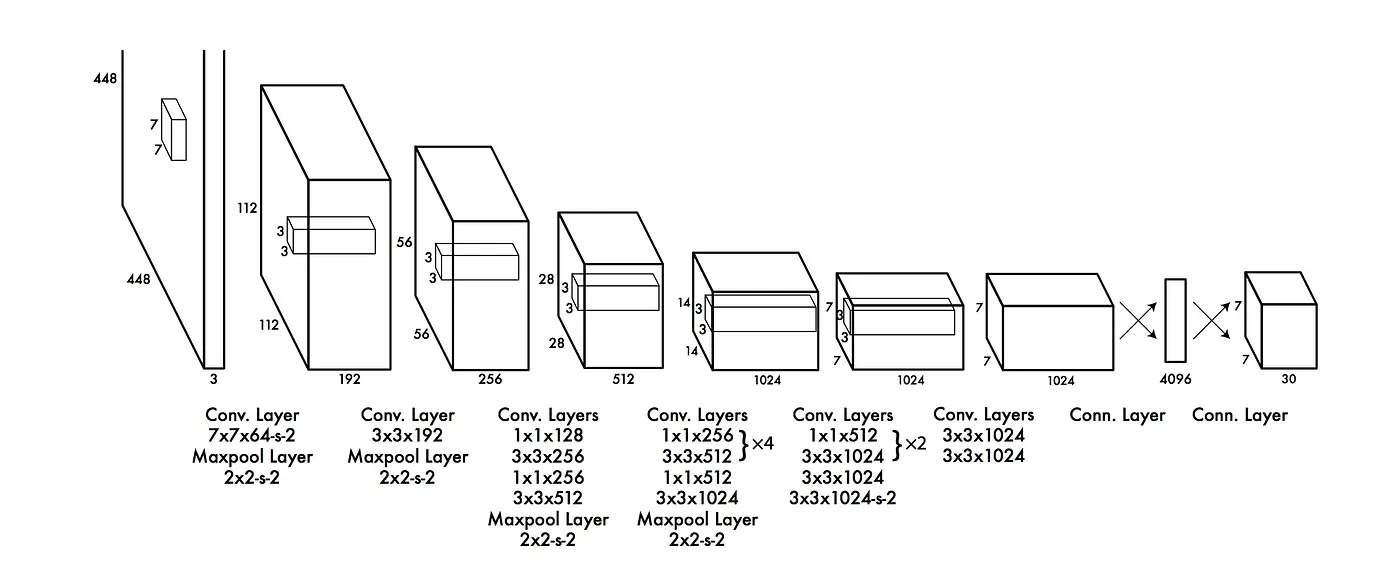
\includegraphics[width=1\textwidth]{files/capitoli/2-yolo/assets/yolov1-architecture.png}
    \caption{\label{fig:yolov1-architecture}Architettura di YOLOv1\cite{17}}
\end{figure}

L'output finale della rete è un tensore di dimensione
\[ S*S*(B*5 + C) \]
dove S è la dimensione della griglia, B è il numero di bounding box predette per cella, e C è il numero di classi. Questo tensore contiene tutte le predizioni delle bounding box, i punteggi di confidenza relativi a ciascuna predizione e le probabilità di classe per ogni oggetto rilevato.

\newpage

\subsection{YOLOv2}
YOLOv2, anche conosciuto come YOLO9000, è stato introdotto nel 2016\cite{18}; questa versione è stata progettata per essere più veloce e precisa, capace di rilevare una gamma più ampia di classi di oggetti.

Le caratteristiche principali includono:
\begin{itemize}
  \item \textbf{Backbone CNN Darknet-19}: YOLOv2 utilizza Darknet-19 come Backbone, una variante dell'architettura VGGNet, con strati di convoluzione progressiva e max-pooling.
  \item \textbf{Anchor Boxes}: introduce le Anchor Boxes, che sono bounding boxes predefinite con diverse proporzioni e scale., le quali permottono al modello di gestire meglio oggetti di varie dimensioni e proporzioni all'interno di un'immagine.
  \item \textbf{Batch Normalization}: l'introduzione della normalizzazione batch standardizza le attivazioni di ogni layer, riducendo il rischio di overfitting e accelerando la convergenza durante l'addestramento. Questo processo aiuta a mantenere l'output di ogni layer stabile e ben bilanciato, facilitando l'apprendimento di feature utili.
  \item \textbf{Strategia di Training Multi-Scale}: viene adottata una strategia di training multi-scala, che consiste nell'addestrare il modello su immagini di diverse scale e risoluzioni. Questa tecnica permette al modello di essere robusto e flessibile, adattandosi meglio a variazioni nelle dimensioni degli oggetti e migliorando la capacità di generalizzazione.
  \item \textbf{Nuova Loss Function}: introdotta una nuova loss function progettata specificamente per l'object detection, la quale è basata sugli errori quadratici tra le bounding box predette e quelle reali, e tiene conto anche delle probabilità di classe. La nuova loss function aiuta il modello a migliorare la precisione delle predizioni, penalizzando in modo appropriato le deviazioni tra le bounding box previste e quelle effettive, e ottimizzando la classificazione degli oggetti rilevati.
\end{itemize}

\begin{figure}[ht]
    \centering
    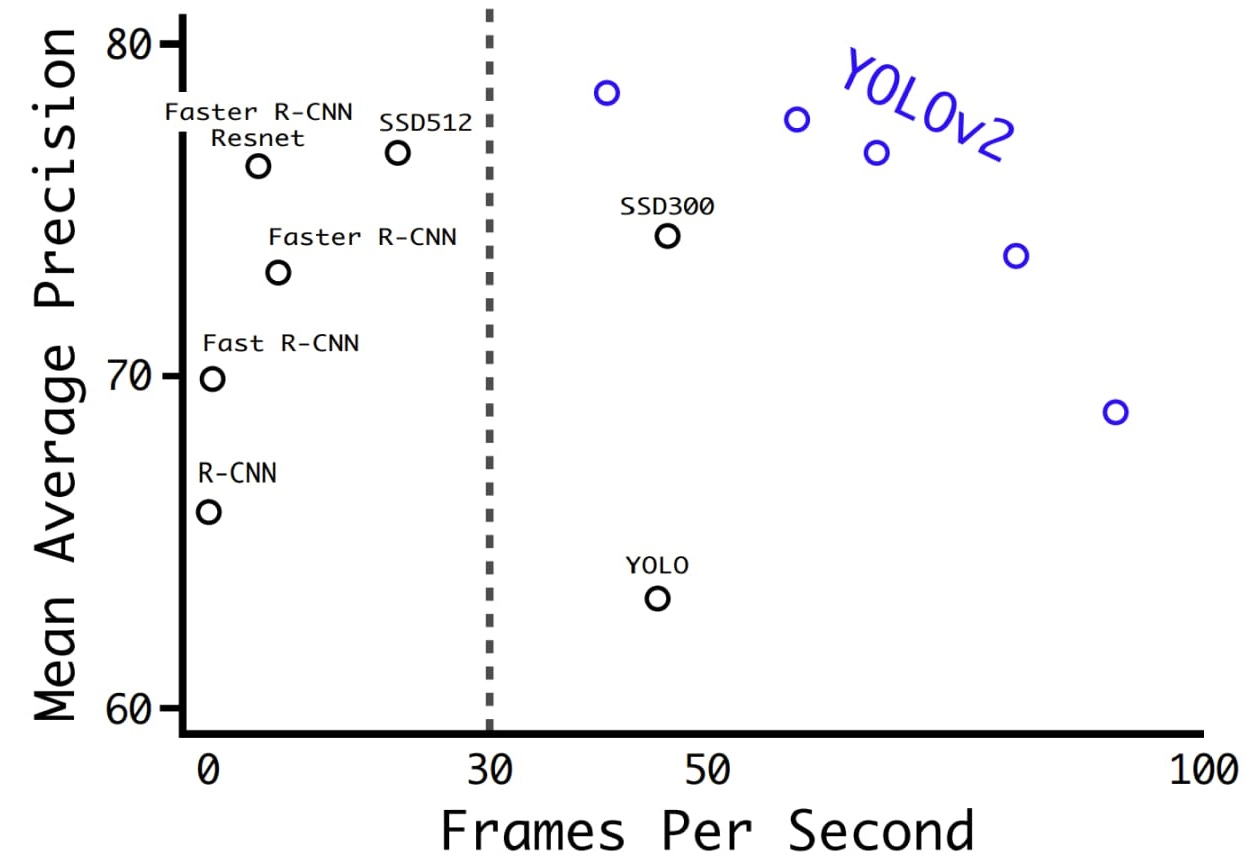
\includegraphics[width=0.7\textwidth]{files/capitoli/2-yolo/assets/yolov2-benchmark.jpeg}
    \caption{\label{fig:yolov2-benchmark}Confronto della mAP di YOLOv2 con quelle di altri modelli\cite{19}}
\end{figure}

\subsection{YOLOv3}
YOLOv3 è la terza versione dell'algoritmo YOLO, introdotta nel 2018\cite{20} con l'obiettivo di aumentare l'accuratezza e la velocità dell'algoritmo. Caratteristiche chiave di YOLOv3 sono:
\begin{itemize}
  \item \textbf{Architettura CNN Darknet-53}: Darknet-53 è una variante dell'architettura ResNet, progettata specificamente per le attività di object detection con 53 convolutional layers.
  \item \textbf{Anchor Boxes migliori}: Implementa anchor boxes scalate e con diversi aspect ratio per adattarsi meglio alle dimensioni e alle forme degli oggetti da rilevare.
  \item \textbf{Feature Pyramid Networks}: Introduce le FPN, una architettura CNN utilizzata per rilevare oggetti a diverse scale, migliorando le prestazioni di detection sugli oggetti di piccole dimensioni.
\end{itemize}

\vspace{1cm}

\begin{figure}[ht]
    \centering
    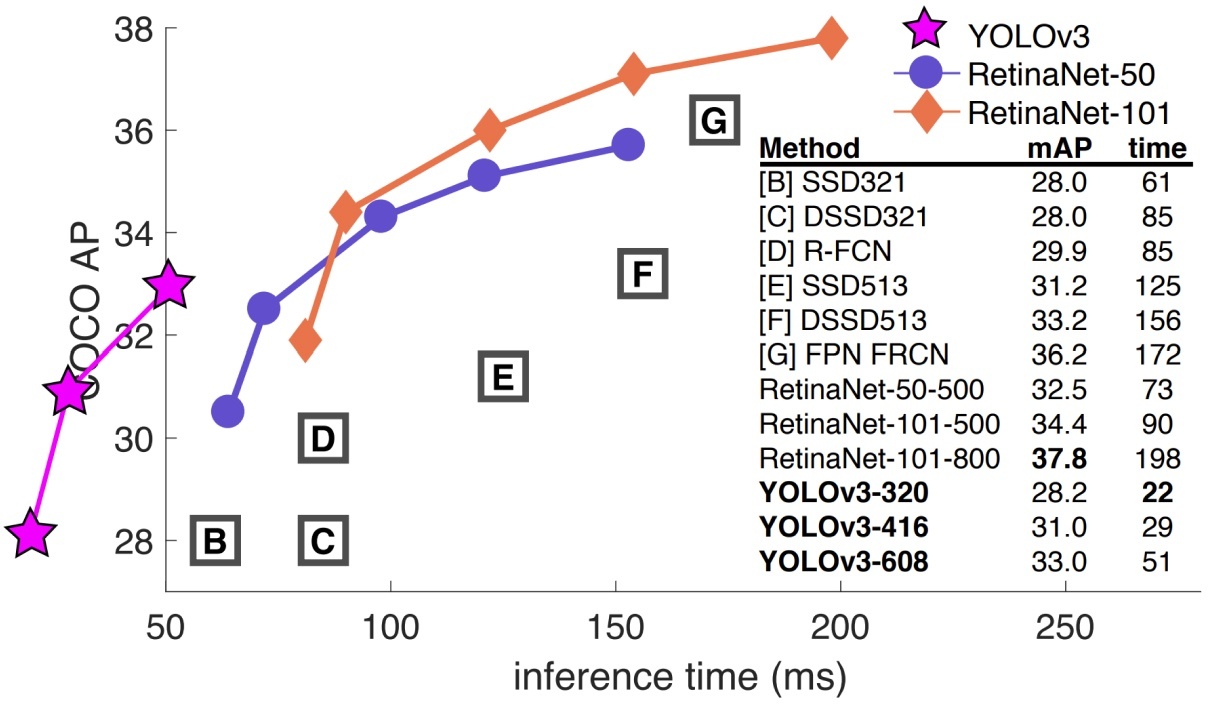
\includegraphics[width=0.8\textwidth]{files/capitoli/2-yolo/assets/yolov3-benchmark.jpeg}
    \caption{\label{fig:yolov3-benchmark}mAP ottenuta su dataset COCO con YOLOv3\cite{19}}
\end{figure}

\subsection{YOLOv4}

YOLOv4 viene rilasciata nel 2020 da Bochkovskiy\cite{21} e presenta le seguenti novità:
\begin{itemize}
  \item \textbf{Architettura CSPNet}: adotta una nuova architettura CNN chiamata CSPNet (Cross Stage Partial Network), una variante della ResNet progettata specificamente per task di object detection.
  \item \textbf{Anchor Box con k-means clustering}: introdotto un nuovo metodo di generazione per le anchor box che sfrutta un algoritmo di clustering per raggruppare le bounding box del ground truth in cluster, utilizzando i centroidi di questi cluster come anchor box; questo permette alle anchor box di essere più precise rispetto alle dimensioni e alla forma degli oggetti rilevati.
  \item \textbf{GHM Loss}: introdotta una variante della Focal Loss, progettata per migliorare le prestazioni del modello su dataset con distribuzione non uniforme delle classi.
  \item \textbf{Miglioramenti alle FPN}: revisione che migliora ulteriormente la capacità del modello di rilevare oggetti di piccole dimensioni, in modo da operare efficacemente su scale diverse all'interno delle immagini.
\end{itemize}

\begin{figure}[ht]
    \centering
    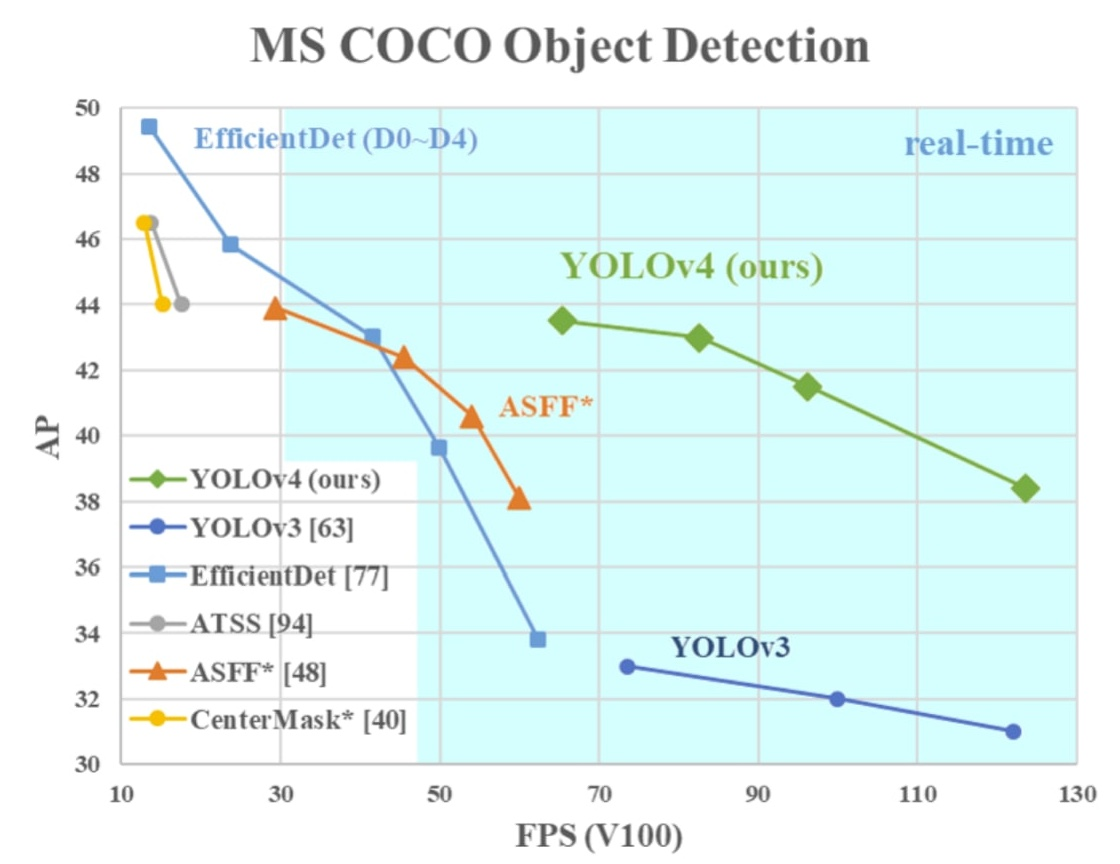
\includegraphics[width=0.8\textwidth]{files/capitoli/2-yolo/assets/yolov4-benchmark.jpeg}
    \caption{\label{fig:yolov4-benchmark}mAP di YOLOv4 confrontata con quelle di modelli precedenti\cite{19}}
\end{figure}

\newpage

\subsection{YOLOv5}
Introdotta nel 2020 dallo stesso team che ha sviluppato l'algoritmo YOLO originale, YOLOv5 è un progetto open-source mantenuto da Ultralytics\cite{22}. Introduce diverse nuove funzionalità e miglioramenti tra cui:
\begin{itemize}
  \item \textbf{Architettura EfficientDet}: utilizza una architettura più complessa chiamata EfficientDet, basata sull'architettura di rete EfficientNet, la quale consente a YOLOv5 di raggiungere una maggiore accuratezza e una migliore generalizzazione su un'ampia gamma di categorie di oggetti rispetto alle versioni precedenti.
  \item \textbf{Addestramento su Dataset Diversificato (D5)}: a differenza di YOLO, che è stato addestrato sul dataset PASCAL VOC composto da 20 categorie di oggetti, YOLOv5 è addestrato su un dataset più ampio e diversificato chiamato D5, che include un totale di 600 categorie di oggetti.
  \item \textbf{Spatial Pyramid Pooling (SPP)}: introduce un nuovo tipo di layer di pooling che riduce la risoluzione spaziale delle feature maps, il quale è particolarmente efficace nel migliorare le prestazioni di rilevamento sugli oggetti di piccole dimensioni, consentendo al modello di analizzare gli oggetti a diverse scale.
   \item \textbf{Loss Function CIoU}: introduce una nuova loss function chiamata "CIoU loss", variante della loss function IoU (Intersection over Union). La CIoU loss è specificamente progettata per migliorare le prestazioni del modello su dataset sbilanciati, contribuendo a migliorare l'accuratezza e la stabilità durante l'addestramento.
\end{itemize}

\newpage

\begin{figure}[ht]
    \centering
    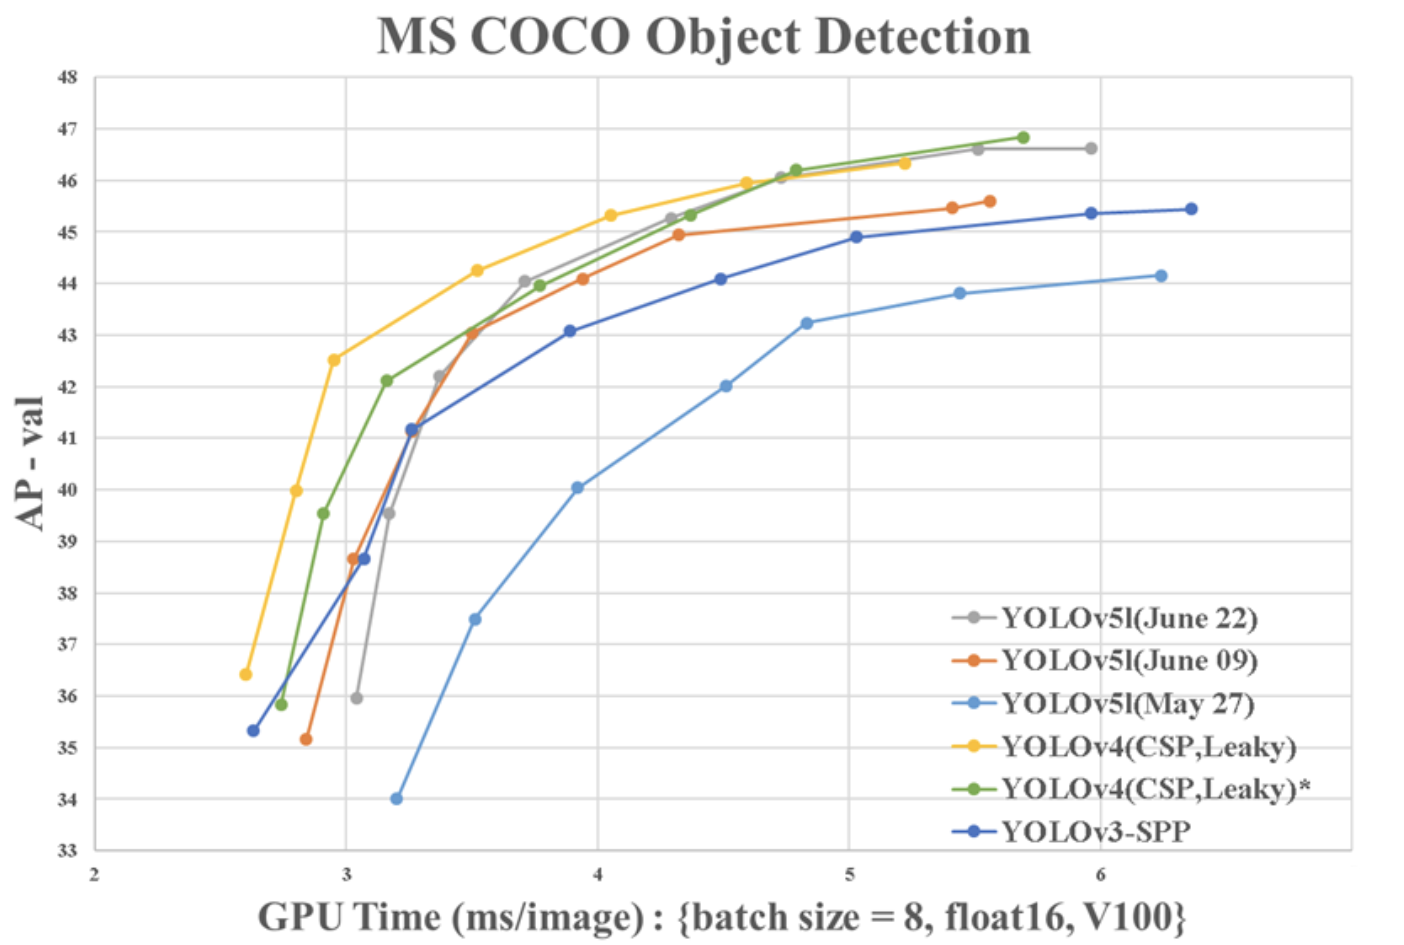
\includegraphics[width=0.9\textwidth]{files/capitoli/2-yolo/assets/yolov5-benchmark.png}
    \caption{\label{fig:yolov5-benchmark}mAP di YOLOv5 confrontata con quelle di modelli precedenti\cite{23}}
\end{figure}

\subsection{YOLOv6}
Proposta nel 2020 da Li et al.\cite{24}, va a migliorare le precedenti versioni introducento una nuova architettura CNN chiamata \textbf{EfficientNet-L2}, una variante dell'architettura EfficientNet che migliora l'efficienza computazionale del modello riducendo il numero di parametri, pur mantenendo elevate prestazioni su vari benchmark di object detection.

\newpage

\subsection{YOLOv7}
La settima versione di YOLO, rilasciata nel 2022 da Chien-Yao Wang, Alexey Bochkovskiy e Hong-Yuan Mark Liao\cite{25}, introduce diverse migliorie significative:
\begin{itemize}
  \item \textbf{Anchor boxes migliorate}: YOLOv7 aumenta a 9 il numero di anchor boxes, il quale permette al modello di rilevare una gamma più ampia di forme e dimensioni degli oggetti rispetto alle versioni precedenti, riducendo così il numero di falsi positivi.
  \item \textbf{Focal Loss}: introdotta una nuova loss function chiamata "focal loss", la quale riduce il peso della loss per esempi ben classificati e si concentran sugli esempi difficili, ovvero gli oggetti difficili da rilevare.
  \item \textbf{Risoluzione più alta e velocità migliorata}: YOLOv7 processa le immagini ad una risoluzione superiore rispetto alle versioni precedenti, ottenendo una precisione complessiva maggiore, ed ad una velocità maggiore, rendendolo adatto per applicazioni sensibili in tempo reale dove velocità di elaborazione più elevate sono cruciali.
\end{itemize}

\newpage